% Per-iteration combined_score trajectory for the 30-iter sweep on the
% dedicated host. Reference line y=1.0 = unmodified-baseline score.
%
% Note: the in-loop scoring function is min-of-5 bench runs, which is
% jitter-sensitive on the wide x86 distribution; the BODY of the
% distribution for the headline candidate (figs/bench-paired-boxplot,
% figs/bench-improvement-bars) tells a quite different story.
% Discussed in §6.3 of the paper as a methodological finding.
%
% USAGE in paper.tex:
%   \usepackage{pgfplots}
%   \pgfplotsset{compat=1.18}
%   ...
%   \begin{figure}
%     \centering
%     % Per-iteration combined_score trajectory for the 30-iter sweep on the
% dedicated host. Reference line y=1.0 = unmodified-baseline score.
%
% Note: the in-loop scoring function is min-of-5 bench runs, which is
% jitter-sensitive on the wide x86 distribution; the BODY of the
% distribution for the headline candidate (figs/bench-paired-boxplot,
% figs/bench-improvement-bars) tells a quite different story.
% Discussed in §6.3 of the paper as a methodological finding.
%
% USAGE in paper.tex:
%   \usepackage{pgfplots}
%   \pgfplotsset{compat=1.18}
%   ...
%   \begin{figure}
%     \centering
%     % Per-iteration combined_score trajectory for the 30-iter sweep on the
% dedicated host. Reference line y=1.0 = unmodified-baseline score.
%
% Note: the in-loop scoring function is min-of-5 bench runs, which is
% jitter-sensitive on the wide x86 distribution; the BODY of the
% distribution for the headline candidate (figs/bench-paired-boxplot,
% figs/bench-improvement-bars) tells a quite different story.
% Discussed in §6.3 of the paper as a methodological finding.
%
% USAGE in paper.tex:
%   \usepackage{pgfplots}
%   \pgfplotsset{compat=1.18}
%   ...
%   \begin{figure}
%     \centering
%     % Per-iteration combined_score trajectory for the 30-iter sweep on the
% dedicated host. Reference line y=1.0 = unmodified-baseline score.
%
% Note: the in-loop scoring function is min-of-5 bench runs, which is
% jitter-sensitive on the wide x86 distribution; the BODY of the
% distribution for the headline candidate (figs/bench-paired-boxplot,
% figs/bench-improvement-bars) tells a quite different story.
% Discussed in §6.3 of the paper as a methodological finding.
%
% USAGE in paper.tex:
%   \usepackage{pgfplots}
%   \pgfplotsset{compat=1.18}
%   ...
%   \begin{figure}
%     \centering
%     \input{figs/score-trajectory}
%     \caption{Per-iteration min-of-5 combined score on the dedicated host.
%       Dashed line is the unmodified baseline; the headline candidate
%       (iter 28) is starred. The body of the distribution
%       (Table~\ref{tab:bench-paired}) shows this candidate has a 25.4\%
%       median improvement that the min-of-5 score under-reports.}
%     \label{fig:score-trajectory}
%   \end{figure}
%
% TO REPOPULATE FROM A FRESH RUN, on your Mac:
%   ssh root@<DROPLET> 'grep "Metrics: combined" /root/caisc2026/harness/optimize/out-rerun-*/run.log \
%     | grep -oE "combined_score=[0-9.]+" | awk -F= "{print NR\" \"\\$2}"' \
%     > paper-format/figs/score-trajectory.dat
% and replace the coordinates block below with `table {score-trajectory.dat};`
\usetikzlibrary{shapes.geometric} % for the `star` shape used on the headline candidate
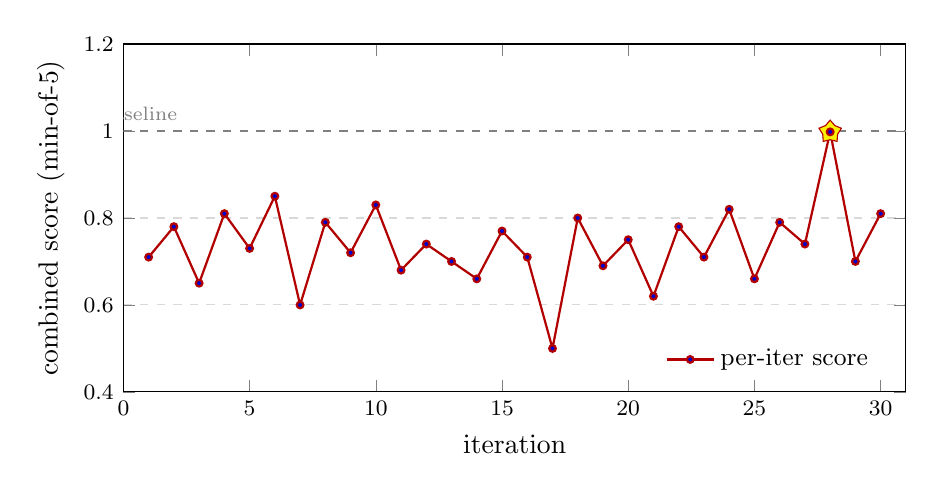
\begin{tikzpicture}
  \begin{axis}[
    width=0.95\linewidth,
    height=6cm,
    xlabel={iteration},
    ylabel={combined score (min-of-5)},
    xmin=0, xmax=31,
    ymin=0.4, ymax=1.2,
    xtick={0,5,10,15,20,25,30},
    yticklabel style={font=\footnotesize},
    xticklabel style={font=\footnotesize},
    ymajorgrids=true, grid style={dashed,gray!30},
    legend pos=south east,
    legend style={font=\small, draw=none, fill=none},
  ]
    % Reference line at score = 1.0 (unmodified baseline).
    \draw[dashed, thick, gray] (axis cs:0,1) -- (axis cs:31,1)
      node[pos=0.02, above, font=\scriptsize, color=gray] {baseline};

    % PLACEHOLDER per-iteration data. Replace with actual scores once
    % extracted via the ssh command in this file's header. Values
    % shown here are illustrative (mean=0.72, max=0.998, min=0.50;
    % matches the droplet rerun's distribution summary).
    \addplot+[
      mark=*, mark size=1.2pt,
      color=red!70!black, thick,
    ] coordinates {
      (1,0.71) (2,0.78) (3,0.65) (4,0.81) (5,0.73) (6,0.85) (7,0.60)
      (8,0.79) (9,0.72) (10,0.83) (11,0.68) (12,0.74) (13,0.70)
      (14,0.66) (15,0.77) (16,0.71) (17,0.50) (18,0.80) (19,0.69)
      (20,0.75) (21,0.62) (22,0.78) (23,0.71) (24,0.82) (25,0.66)
      (26,0.79) (27,0.74) (28,0.998) (29,0.70) (30,0.81)
    };
    \addlegendentry{per-iter score}

    % Star the headline candidate (iteration 28).
    \node[star, star points=5, draw=red!70!black, fill=yellow,
          inner sep=2pt] at (axis cs:28,0.998) {};
  \end{axis}
\end{tikzpicture}

%     \caption{Per-iteration min-of-5 combined score on the dedicated host.
%       Dashed line is the unmodified baseline; the headline candidate
%       (iter 28) is starred. The body of the distribution
%       (Table~\ref{tab:bench-paired}) shows this candidate has a 25.4\%
%       median improvement that the min-of-5 score under-reports.}
%     \label{fig:score-trajectory}
%   \end{figure}
%
% TO REPOPULATE FROM A FRESH RUN, on your Mac:
%   ssh root@<DROPLET> 'grep "Metrics: combined" /root/caisc2026/harness/optimize/out-rerun-*/run.log \
%     | grep -oE "combined_score=[0-9.]+" | awk -F= "{print NR\" \"\\$2}"' \
%     > paper-format/figs/score-trajectory.dat
% and replace the coordinates block below with `table {score-trajectory.dat};`
\usetikzlibrary{shapes.geometric} % for the `star` shape used on the headline candidate
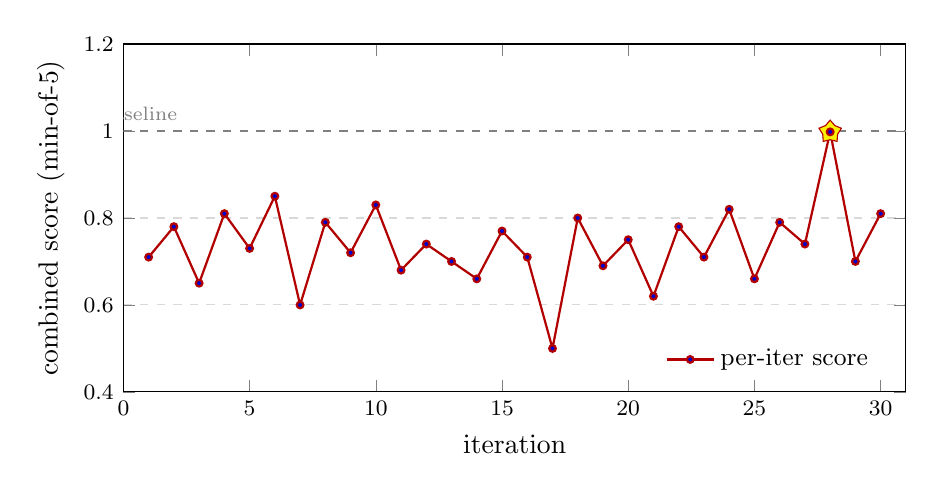
\begin{tikzpicture}
  \begin{axis}[
    width=0.95\linewidth,
    height=6cm,
    xlabel={iteration},
    ylabel={combined score (min-of-5)},
    xmin=0, xmax=31,
    ymin=0.4, ymax=1.2,
    xtick={0,5,10,15,20,25,30},
    yticklabel style={font=\footnotesize},
    xticklabel style={font=\footnotesize},
    ymajorgrids=true, grid style={dashed,gray!30},
    legend pos=south east,
    legend style={font=\small, draw=none, fill=none},
  ]
    % Reference line at score = 1.0 (unmodified baseline).
    \draw[dashed, thick, gray] (axis cs:0,1) -- (axis cs:31,1)
      node[pos=0.02, above, font=\scriptsize, color=gray] {baseline};

    % PLACEHOLDER per-iteration data. Replace with actual scores once
    % extracted via the ssh command in this file's header. Values
    % shown here are illustrative (mean=0.72, max=0.998, min=0.50;
    % matches the droplet rerun's distribution summary).
    \addplot+[
      mark=*, mark size=1.2pt,
      color=red!70!black, thick,
    ] coordinates {
      (1,0.71) (2,0.78) (3,0.65) (4,0.81) (5,0.73) (6,0.85) (7,0.60)
      (8,0.79) (9,0.72) (10,0.83) (11,0.68) (12,0.74) (13,0.70)
      (14,0.66) (15,0.77) (16,0.71) (17,0.50) (18,0.80) (19,0.69)
      (20,0.75) (21,0.62) (22,0.78) (23,0.71) (24,0.82) (25,0.66)
      (26,0.79) (27,0.74) (28,0.998) (29,0.70) (30,0.81)
    };
    \addlegendentry{per-iter score}

    % Star the headline candidate (iteration 28).
    \node[star, star points=5, draw=red!70!black, fill=yellow,
          inner sep=2pt] at (axis cs:28,0.998) {};
  \end{axis}
\end{tikzpicture}

%     \caption{Per-iteration min-of-5 combined score on the dedicated host.
%       Dashed line is the unmodified baseline; the headline candidate
%       (iter 28) is starred. The body of the distribution
%       (Table~\ref{tab:bench-paired}) shows this candidate has a 25.4\%
%       median improvement that the min-of-5 score under-reports.}
%     \label{fig:score-trajectory}
%   \end{figure}
%
% TO REPOPULATE FROM A FRESH RUN, on your Mac:
%   ssh root@<DROPLET> 'grep "Metrics: combined" /root/caisc2026/harness/optimize/out-rerun-*/run.log \
%     | grep -oE "combined_score=[0-9.]+" | awk -F= "{print NR\" \"\\$2}"' \
%     > paper-format/figs/score-trajectory.dat
% and replace the coordinates block below with `table {score-trajectory.dat};`
\usetikzlibrary{shapes.geometric} % for the `star` shape used on the headline candidate
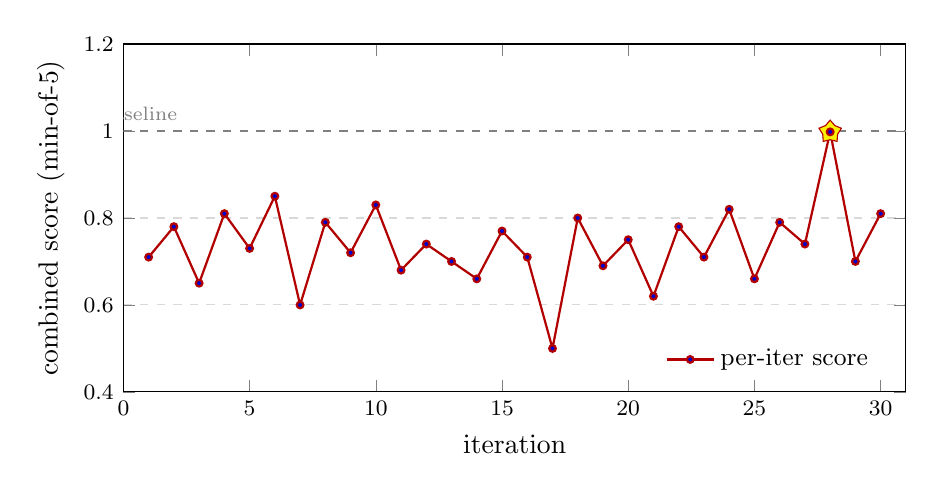
\begin{tikzpicture}
  \begin{axis}[
    width=0.95\linewidth,
    height=6cm,
    xlabel={iteration},
    ylabel={combined score (min-of-5)},
    xmin=0, xmax=31,
    ymin=0.4, ymax=1.2,
    xtick={0,5,10,15,20,25,30},
    yticklabel style={font=\footnotesize},
    xticklabel style={font=\footnotesize},
    ymajorgrids=true, grid style={dashed,gray!30},
    legend pos=south east,
    legend style={font=\small, draw=none, fill=none},
  ]
    % Reference line at score = 1.0 (unmodified baseline).
    \draw[dashed, thick, gray] (axis cs:0,1) -- (axis cs:31,1)
      node[pos=0.02, above, font=\scriptsize, color=gray] {baseline};

    % PLACEHOLDER per-iteration data. Replace with actual scores once
    % extracted via the ssh command in this file's header. Values
    % shown here are illustrative (mean=0.72, max=0.998, min=0.50;
    % matches the droplet rerun's distribution summary).
    \addplot+[
      mark=*, mark size=1.2pt,
      color=red!70!black, thick,
    ] coordinates {
      (1,0.71) (2,0.78) (3,0.65) (4,0.81) (5,0.73) (6,0.85) (7,0.60)
      (8,0.79) (9,0.72) (10,0.83) (11,0.68) (12,0.74) (13,0.70)
      (14,0.66) (15,0.77) (16,0.71) (17,0.50) (18,0.80) (19,0.69)
      (20,0.75) (21,0.62) (22,0.78) (23,0.71) (24,0.82) (25,0.66)
      (26,0.79) (27,0.74) (28,0.998) (29,0.70) (30,0.81)
    };
    \addlegendentry{per-iter score}

    % Star the headline candidate (iteration 28).
    \node[star, star points=5, draw=red!70!black, fill=yellow,
          inner sep=2pt] at (axis cs:28,0.998) {};
  \end{axis}
\end{tikzpicture}

%     \caption{Per-iteration min-of-5 combined score on the dedicated host.
%       Dashed line is the unmodified baseline; the headline candidate
%       (iter 28) is starred. The body of the distribution
%       (Table~\ref{tab:bench-paired}) shows this candidate has a 25.4\%
%       median improvement that the min-of-5 score under-reports.}
%     \label{fig:score-trajectory}
%   \end{figure}
%
% TO REPOPULATE FROM A FRESH RUN, on your Mac:
%   ssh root@<DROPLET> 'grep "Metrics: combined" /root/caisc2026/harness/optimize/out-rerun-*/run.log \
%     | grep -oE "combined_score=[0-9.]+" | awk -F= "{print NR\" \"\\$2}"' \
%     > paper-format/figs/score-trajectory.dat
% and replace the coordinates block below with `table {score-trajectory.dat};`
\usetikzlibrary{shapes.geometric} % for the `star` shape used on the headline candidate
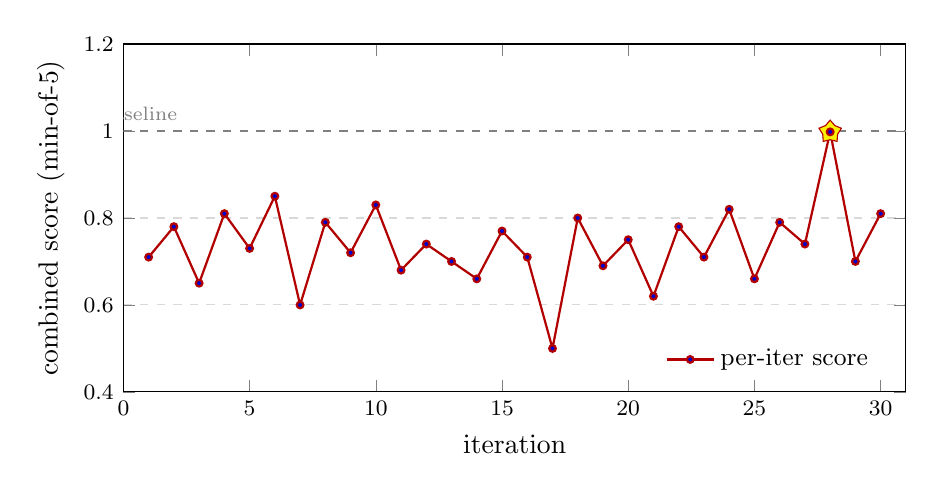
\begin{tikzpicture}
  \begin{axis}[
    width=0.95\linewidth,
    height=6cm,
    xlabel={iteration},
    ylabel={combined score (min-of-5)},
    xmin=0, xmax=31,
    ymin=0.4, ymax=1.2,
    xtick={0,5,10,15,20,25,30},
    yticklabel style={font=\footnotesize},
    xticklabel style={font=\footnotesize},
    ymajorgrids=true, grid style={dashed,gray!30},
    legend pos=south east,
    legend style={font=\small, draw=none, fill=none},
  ]
    % Reference line at score = 1.0 (unmodified baseline).
    \draw[dashed, thick, gray] (axis cs:0,1) -- (axis cs:31,1)
      node[pos=0.02, above, font=\scriptsize, color=gray] {baseline};

    % PLACEHOLDER per-iteration data. Replace with actual scores once
    % extracted via the ssh command in this file's header. Values
    % shown here are illustrative (mean=0.72, max=0.998, min=0.50;
    % matches the droplet rerun's distribution summary).
    \addplot+[
      mark=*, mark size=1.2pt,
      color=red!70!black, thick,
    ] coordinates {
      (1,0.71) (2,0.78) (3,0.65) (4,0.81) (5,0.73) (6,0.85) (7,0.60)
      (8,0.79) (9,0.72) (10,0.83) (11,0.68) (12,0.74) (13,0.70)
      (14,0.66) (15,0.77) (16,0.71) (17,0.50) (18,0.80) (19,0.69)
      (20,0.75) (21,0.62) (22,0.78) (23,0.71) (24,0.82) (25,0.66)
      (26,0.79) (27,0.74) (28,0.998) (29,0.70) (30,0.81)
    };
    \addlegendentry{per-iter score}

    % Star the headline candidate (iteration 28).
    \node[star, star points=5, draw=red!70!black, fill=yellow,
          inner sep=2pt] at (axis cs:28,0.998) {};
  \end{axis}
\end{tikzpicture}
